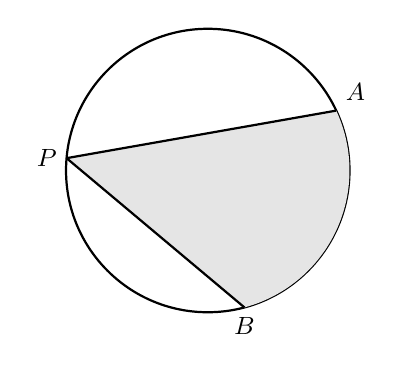
\begin{tikzpicture}[>=latex, font=\small, scale=1.0]
  \coordinate (O) at (0, 0);
  \draw[thick] (O) circle (1.8cm);

  \coordinate (P) at (175:1.8);
  \coordinate (A) at (25:1.8);
  \coordinate (B) at (285:1.8);

  % 阴影区域：弦 PA、PB 及右侧圆弧围成的区域
  \fill[gray!20] (P) -- (A) arc (25:-75:1.8cm) -- cycle;

  \draw[thick] (P) -- (A);
  \draw[thick] (P) -- (B);

  \node[left] at (P) {$P$};
  \node[above right] at (A) {$A$};
  \node[below] at (B) {$B$};
\end{tikzpicture}
